\documentclass[12pt]{report}
\usepackage[utf8x]{inputenc}
\usepackage[russian]{babel}
\usepackage{amsmath}
\usepackage{graphicx}

\graphicspath{{graphic/chapter3/}}

\renewcommand{\labelenumii}{\arabic{enumi}.\arabic{enumii}}

\textwidth=15cm
\textheight=22cm
\oddsidemargin= 0.5cm
\topmargin = -0.5cm


\begin{document}
\chapter{Разработка системы моделирования.}
    \section{Разработка архитектуры приложения. }
    Разрабатываемая система позволяет пользователю строить  модель локальной сети, используя объекты, имитирующие различное сетевое оборудование, проводить эксперименты в различных режимах работы, анализировать полученные результаты. Каждая из этих возможностей может быть реализована посредством подсистемы, которые являются компонентами проектируемой системы. Таким образом можно выделить следующие подсистемы.

    \begin{itemize}
        \item Подсистема моделирования. Данная подсистема отвечает за правильное взаимодействие компонентов модели, учитывая их параметры.
        \item Подсистема управления отвечает за сохранение(загрузку) параметров моделей, создание модели сети, а так же предоставляет методы для ее функционирования.
        \item Подсистема мониторинга отвечает за сбор данных в процессе моделирования и их анализ
    \end{itemize}

    Взаимодействие данных подсистем представлено на рисунке ().

    \subsection{Подсистема моделирования. }

    Для реализации подсистемы моделирования необходимо описать взаимодействие различных компонент, входящих в ее состав. Такими компонентами являются модели устройств, протоколов, приложений. Объединение сетевых устройств в проектируемой системе посредством моделей сетевых соединений. Модель локальной сети представляет собой совокупность моделей устройств и их взаимодействия.

    \subsubsection{Канал связи. }

    Для имитации передачи данных могут быть использованы различные модели канала связи. При использовании модели идеального канала без помех единственной характеристикой такого соединения является задержка при передачи данных. В случае необходимости анализа передачи данных в каналах связи с помехами необходима реализация алгоритма генерации помехи. Используемая в системе модель канала связи представлена на рисунке~\ref{Pic2}.

    \begin{figure}[h!]\center
        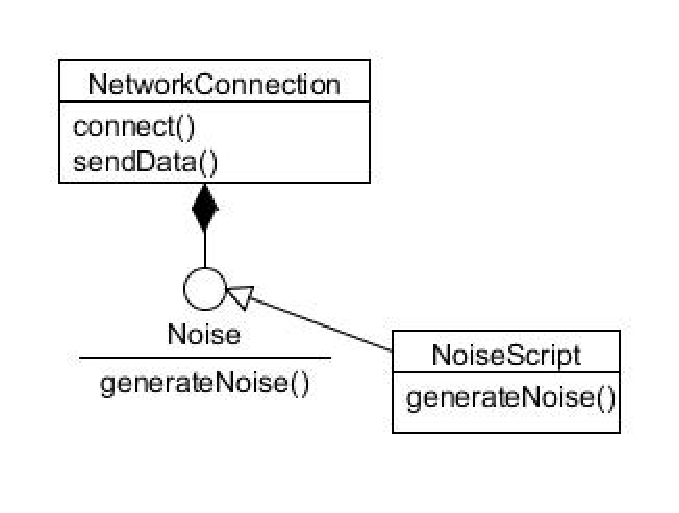
\includegraphics[width = 60mm]{Ch3Pic2}
        \caption{Диаграмма классов модели канала связи. } \label{Pic2}
    \end{figure}

    Класс NoiseScript описывает алгоритм генерации помехи и связан с моделью канала связи через интерфейс Noise. Такая архитектура позволяет изменять использую модель канала связи без внесения изменений в архитектуру приложения.

    \subsubsection{Протоколы. }

    Для использования при моделировании различных сетевых протоколов они разбиты на четыре группы. К первой группе относятся протоколы, обрабатывающие данные приложений или вышестоящих протоколов. Каждый протокол, относящийся к этой группе, выполняет разделение данных на части и дополняет их служебными полями. В проектируемой модели, использующей стек протоколов TCP/IP, для каждого протокола эти фрагменты данных называются по-разному. Для Ethernet - кадры, для IP - пакеты, для TCP - сегменты. Структура взаимодействия протоколов отражена на рисунке~\ref{Pic3}.

    \begin{figure}[h!]\center
        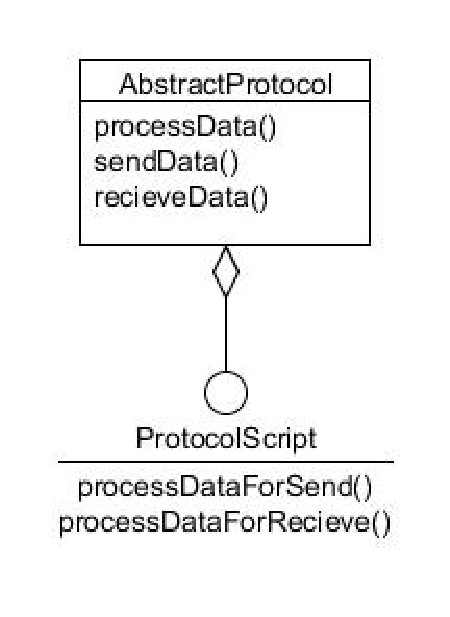
\includegraphics[width = 40mm]{Ch3Pic3}
        \caption{Диаграмма классов модели протокола. } \label{Pic3}
    \end{figure}

    Анализ служебных полей фрагмента данных описывается в классе, реализующем интерфейс ProtocolScript. Данный механизм позволяет описывать различные протоколы для использования в системе, однако осложняет архитектуру приложения и описание процесса взаимодействия протокола.

    Второй группой протоколов, выделенных на этапе моделирования, являются протоколы управления средой. В стеке протоколов TCP/IP таким протоколом является протокол MAC-подуровня, уровня передачи данных. Отличительной особенностью этих протоколов является связь с устройством передачи данных и возможность контроля за передачей. На рисунке~\ref{Pic4} изображена диаграмма классов, используемая для описания этой группы протоколов.

    \begin{figure}[h!]\center
        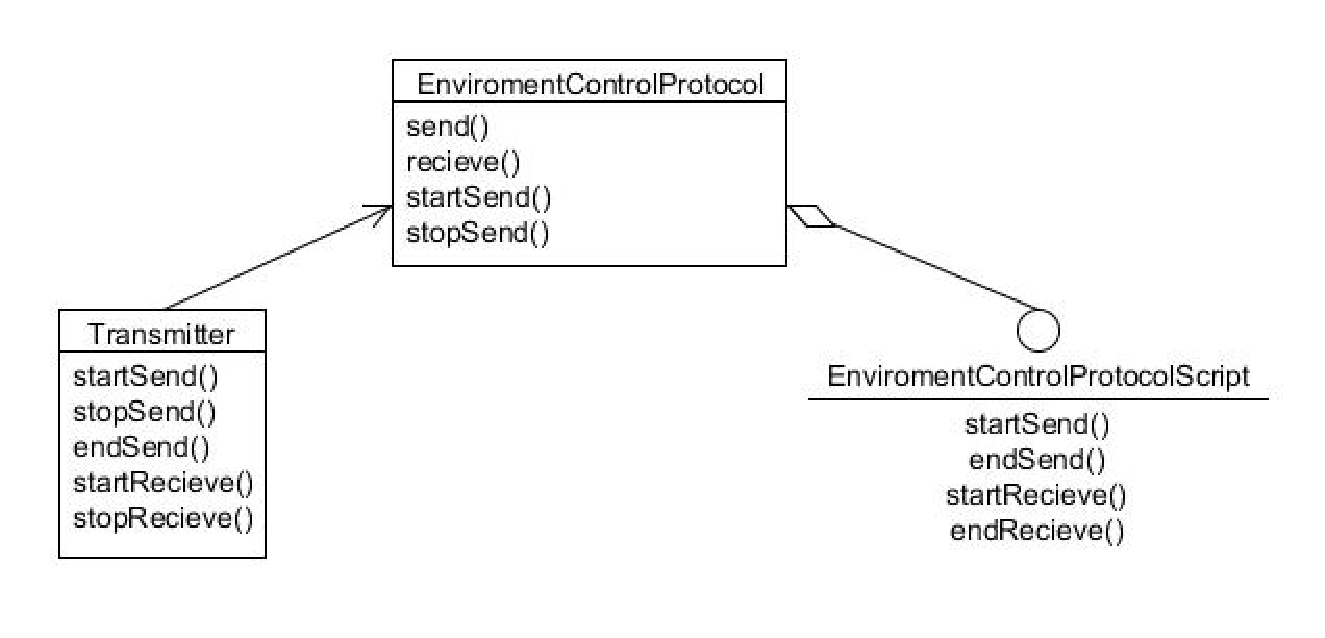
\includegraphics[width = 100mm]{Ch3Pic4}
        \caption{Диаграмма классов модели протокола управления средой. } \label{Pic4}
    \end{figure}

    Интерфейс EnviromentControlProtocolScript предоставляет возможность описания различных протоколов управления средой. Для разрабатываемой модели будет реализован метод доступа с контролем несущей и обнаружением коллизий. Данный метод не используется в современных сетях с дуплексным каналом обмена информацией, однако необходим при использовании полудуплексного режима обмена данными.

    Алгоритм, описанный в классе EnviromentControlProtocolScript, определяет возможно ли начать передачу в данный момент времени, возможно ли считать передачу или прием данных успешными и, в некоторых случаях, определяет задержку передачи данных.

    Устройство передачи данных не выполняет никаких действий по контролю за процессом передачи данных, и является моделью передатчика, который генерирует необходимый сигнал и передает его в канал связи.

    Третьей группой протоколов являются служебные протоколы. В стеке протоколов TCP/IP таким протоколом является ARP. Он используется для установления соответствия между физическими адресами и адресами, используемыми на более высоком уровне модели. Для использования этого протокола необходимо внести изменения в архитектуру протоколов первой группы. Для этого добавляется еще один метод для отправки данных, использование которого сопряжено с запросом адреса, используемого на более низком уровне модели, соответствующего адресу на данном уровне. Взаимодействие протоколов первой группы и служебного протокола изображено на рисунке~\ref{Pic5}.
    
    \begin{figure}[h!]\center
        \includegraphics[width = 100mm]{Ch3Pic5}
        \caption{Схема взаимодействия протоколов передачи данных и служебного протокола. } \label{Pic5}
    \end{figure}
    
    Протоколы первой и третьей группы являются экземплярами одного и того же класса, который был расширен методами для операций по установлению соответствия адресов. Для подобного рода операций, служебные протоколы связаны с протоколами более низкого уровня, что позволяет им взаимодействовать независимо от адресов более высоких уровней модели. 
    
    К четвертой группе протоколов относятся протоколы, связанные с приложениями. Данный вид протоколов предоставляет приложению интерфейс для обмена данными посредством локальной сети. В рамках используемой модели это протоколы четвертого уровня, содержащие в себе операции транспортного уровня, уровня представления данных и сеансового уровня. Учитывая сложность данных процессов, при реализации протокола TCP было принято решение выделить необходимые операции в отдельную подсистему. Диаграмма классов данной подсистемы представлена на рисунке~\ref{Pic6}.
    
    \begin{figure}[h!]\center
        \includegraphics[width = 100mm]{Ch3Pic6}
        \caption{Диаграмма классов транспортной подсистемы. } \label{Pic6}
    \end{figure}
    
    Интерфейс UserTransportFace предоставляет приложению методы для взаимодействия с транспортной подсистемой. Класс ConnectionControlSubsystem отвечает за установление, поддержание и закрытие TCP соединения. В этом классе определяются алгоритмы обработки данных в зависимости от состояния в котором находится соединение. Схема состояний и переходов представлена на рисунке~\ref{Pic7}. На данном уровне абстракции используется понятие сегмента данных. Начальное состояние системы - CLOSED. Управление соединением происходит посредством команд, поступающих от приложения и принятых служебных сегментов. 
    
    

    \begin{figure}[h!]\center
        \includegraphics[width = 100mm]{Ch3Pic7}
        \caption{Схема конечного автомата TCP-соединения. } \label{Pic7}
    \end{figure}    
    

    Типичный случай клиента, активно соединяющегося с сервером показан на жирными линиями - сплошными для клиента, прерывистыми для сервера. Тонкие линии обозначают необычные последовательности событий. Каждая линия маркирована парой событие/действие. Событие может представлять собой либо обращение пользователя к системной процедуре(CONNECT, LISTEN, SEND или CLOSE), либо прибытие сегмента(SYN, FIN, ACK, RST), либо, в одном случае, окончание периода ожидания, равного двойному времени жизни пакета. Действие может состоять в отправке управляющего сегмента(SYN, FIN или RST). Системные процедуры имеют следующее назначение:
    \begin{itemize}
        \item LISTEN - переводит систему в состояние ожидания соединений.
        \item CONNECT - попытка активного создания соединения.
        \item SEND - отправка данных.
        \item CLOSE - закрытие соединения.
    \end{itemize}
    
    Управляющие сегменты имеют следующее назначение:
    
    \begin{itemize}
        \item SYN - сегмент, отправляемый при установлении соединения. 
        \item FIN - сегмент, отправляемый при закрытии соединения.
        \item RST - сегмент, отправляемый при сбросе соединения.
        \item ACK - сегмент, отправляемый для подтверждения получения определенного сегмента.
    \end{itemize}
    
    Назначение того или иного сегмента определяется наличием или отсутствием того или иного флага в TCP-заголовке сегмента. 
    
    Класс SegmentControlSubSystem отвечает за гарантированную доставку сообщений. Это достигается за счет отправки сегмента данных до тех пор, пока не будет получено подтверждение об успешном его приеме. 

    \subsubsection{Модели приложений.}
    
    Приложения, использованные в системе для моделирования действий пользователя, могут использовать протоколы разных уровней. Алгоритмы маршрутизации, используемые в коммутаторах и маршрутизаторах работают на сетевом уровне, как и алгоритмы генерации трафика. Модели уязвимостей используют транспортную подсистему. 
    
    Приложение, используемое в коммутаторе, представляет собой алгоритм определения соединения, через которое будет направлен полученный пакет. Данный алгоритм имеет два режима работы. Первый - это режим обучения. В этом режиме составляется таблица соответствия физического адреса и порта коммутатора, к которому подключен абонент. При этом полученный пакет передается через все активные порты. Второй режим работы использует построенную на первом этапе таблицу маршрутизации для передачи пакета только указанному получателю. Исключением является широковещательный трафик. 
    
        %Алгоритм работы маршрутизатора
    
    
        %Генераторы трафика. 
    
    Для моделирования процесса атаки на рабочую станцию, связанного с наличием уязвимости в приложении используем описанную модель активов и уязвимостей. Уязвимость отличается от актива только тем, что в случае удачной атаки, система считается скомпрометированной в то время, как удачная атака на один из активов подразумевает только получение некоторой информации. Для атаки на приложение злоумышленнику необходимо установить TCP-соединение с целевой рабочей станцией и послать соответствующий запрос. Приложение обрабатывает запрос и, с учетом параметров, влияющих на вероятность успеха, либо возвращает некоторую информацию, либо пустое значение, что означает, что атака была неудачной. Диаграмма классов, описывающая взаимодействие моделей приложений и транспортной подсистемы показана на рисунке~\ref{Pic8}

    \begin{figure}[h!]\center
        \includegraphics[width = 100mm]{Ch3Pic8}
        \caption{Диаграмма классов модели пользовательского приложения. } \label{Pic8}
    \end{figure}    

    Абстрактный класс Application отвечает за загрузку и передачу данных уязвимостям(Vulnerability) и активам(Asset). Для реализации некоторого приложения, алгоритм его действий необходимо реализовать в классе-наследнике класса Application. На приведенном рисунке таким классом является ListenPortApplication. Данный класс создает TCP-сокет и переводит его в режим ожидания входящего соединения. Подобное поведение наиболее удобно для демонстрации процесса атаки, однако возможна реализация и более сложных алгоритмов. 
    
    Модель поведения злоумышленника так же описывается в классе-наследнике от Application. При этом необходимо описать процесс формирования данных, которые будут отправлены приложению-жертве. В эти данные входит так же и параметры атакующего, такие как мотивация и уровень знаний. 
    
    Каждая модель уязвимости или актива содержит таблицу, в которой хранятся вероятности успеха атаки в зависимости от характеристик атакующего и таблицу необходимой для успешной атаки информации, которая должна содержаться в сообщении злоумышленника. 
    
    Таким образом, диаграмма классов, описывающая структуру модели сетевого устройства может быть изображена следующим образом(рисунок~\ref{Pic9}). Представленное изображение является упрощенным представлением архитектуры модели используемой в приложении. На нем отсутствуют вспомогательные классы, выполняющие различные операции с данными, суть которых не влияет на процесс обработки информации в целом.

    \begin{figure}[pH]\center
        \includegraphics[width = 140mm]{Ch3Pic9}
        \caption{Диаграмма классов модели сетевого устройства. } \label{Pic9}
    \end{figure}    

    \subsection{Подсистема управления}
    
    Подсистема управления обеспечивает создание модели, ее функционирование, и является посредником между моделью и пользовательским интерфейсом, а так же подсистемой моделирования. Создание модели может производится двумя путями. Первый заключается в создании модели с помощью пользовательского интерфейса. При этом, оперируя готовыми моделями устройств и их настройками, возможно создание сетей различных конфигураций. Параметры моделей устройств хранятся в файлах XML, данные в которых разделены по подгруппам. Каждый файл отвечает за объекты, относящиеся к одной группе моделей. Такими группами являются модели приложений, модели стека протоколов, модели устройств. Таким образом модель конечного устройства, которая будет использоваться при моделировании, собирается из разных компонент, за загрузку которых отвечают классы NetworkConfigurationLoader, ApplicationManager. Параметры сетевых устройств, такие как адреса, загружаются классом Network в процессе создания сети. Для связывания данных, хранящихся в XML-файлах и объектов в программе используется набор интерфейсов, который называется JAXB(Java Architecture for XML Binding).
    
    \section{Описание работы приложения}
    %Архитектура
        %Разработка объектов моделей
            %Канал связи
            %Протокол
                %Используемые протоколы Ethernet, IP, ARP, TCP
                %Транспортная подсистема
                    %Сокеты, подсистемы управления соединением и сегментами.
            %Стек протоколов (удалено)
                %Принцип взаимодействия. Диаграмма классов. (удалено)
            %Приложения для разных уровней
                %Приложения, использующие IP 
                    %Генераторы пользователького трафика
                    %Генераторы для моделирования DDoS, spoofing etc                
                %Приложения, использующие транспортную подсистему
                    %Приложения - assets
                    %Приложения - Vulnerabilities
                    %Приложения - Поведение злоумышленника
        %Разработка общей модели предметной области 
            %Картинка общей архитектуры модели
            %Принцип работы. 
        %Разработка системы управления  
            %Используемые форматы для хранения данных 
            %Разработка пользовательского интерфейса
                %Драг н дроп
                %Заготовки устройств 
                %Алгоритм отображения графа
        %Разработка системы мониторинга
            %Используемая библиотека
            %Системы мониторов 
            %Система сбора данных
            %Система статистической обработки данных
        %Общий вид архитектуры приложения 
            %Картинка с пояснениями.

    %Софт. Тестирование. Скриншоты. Возможности. 
        %Создание модели
        %Сохранение модели
        %Эксперименты с моделью(показать, что можно принимать меры: антивирусы, межсетевые экраны.)
            %Нормальный режим
            %Спуфинг
            %ДДоС атака
            %Тестирование на проникновение
        %Анализ производительности
        %Выводы
        %Перспективы.
\end{document} 